\section{Introduction}
\label{sec:intro}

In order to achieve certain performance goals, software engineers must often
design systems where the owners of the data being processed are different from
the owners of the computing infrastructure used to process the data, who in
turn might be different from the suppliers of the software that processes the
data. This raises the problem that the data owner must trust both the owner
of the computing infrastructure and the software supplier to handle the data
according to some privacy policy.

\begin{figure}[hbtp]
  \centering
  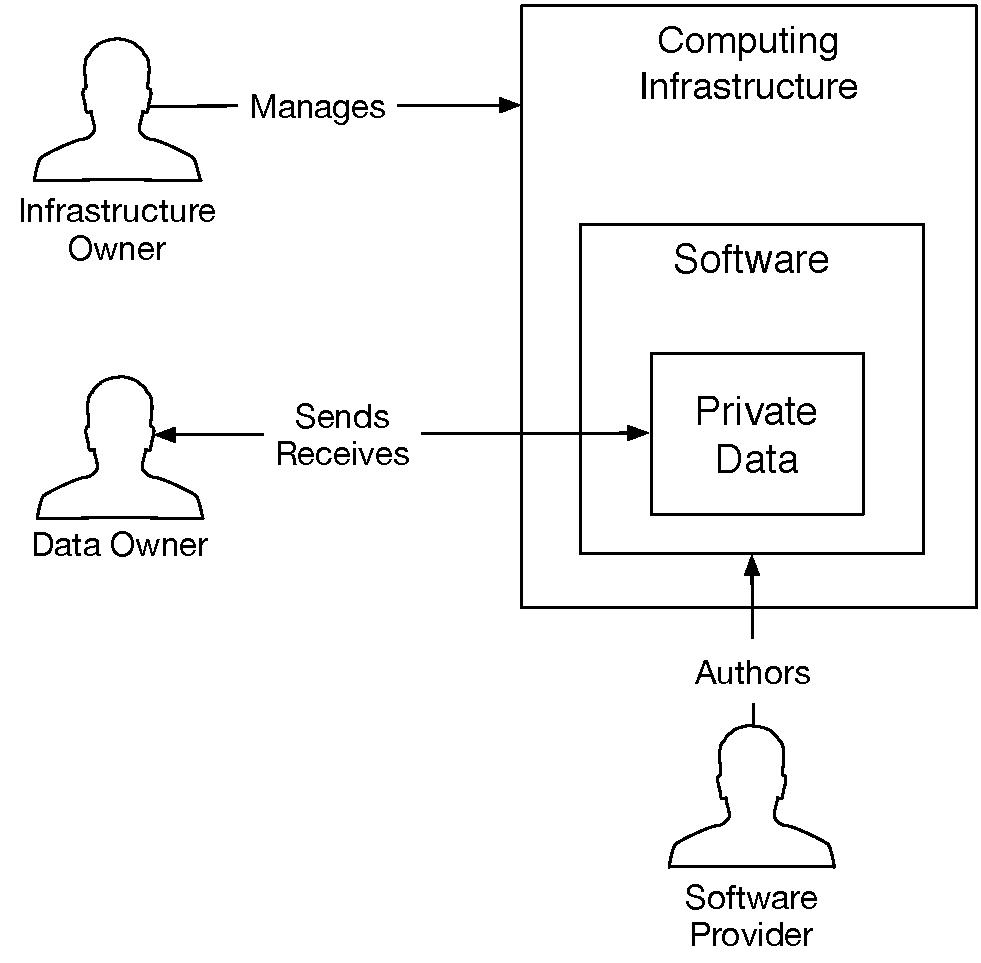
\includegraphics[width=75mm]{figures/computing_model.pdf}
  \caption{
    The computing model assumed by our system. The infrastructure owner,
    software provider and data owner mutually distrust each other. Our system
    aims to guarantee that the private data will not leak even if the software
    is malicious and cooperates with a malicious infrastructure, or with
    another malicious piece of software running on the infrastructure.
  }
  \label{fig:computing_model}
\end{figure}

\subsection{Motivation}
\label{sec:motivation}

The most popular instance of the above problem is cloud computing using public
clouds. For example, CheapoTax, a software provider, might provide tax return
preparation software as a service running on Amazon's public cloud. Users
upload their financial information, encrypted using TLS, to Amazon data
centers, where CheapoTax's computation uses the data to produce tax returns,
which are downloaded by the users in an encrypted form, using TLS. Currently,
the users must trust that neither Amazon nor CheapoTax will record their
private financial information. Users must also hope that neither Amazon's
infrastructure nor CheapoTax's software have bugs that would allow other rogue
actors to obtain the private financial data by running malicious software in
the same public Amazon cloud used by CheapoTax.

Another example of the problem we are aiming to solve is a multiplayer game of
any genre, such as League of Legends \cite{riot2009lol},
World of Warcraft \cite{blizzard2004wow}, StarCraft \cite{blizzard2010sc2}, and
Doom \cite{id2004doom}. The gameplay of many multiplayer games, such as the
ones listed above, rely on the fact that that players can only access a subset
of the game state that is dictated by the units they control. To compensate for
network latencies, many games entrust a player's game client with a superset
of the game state that the user should have access to. For example, in
StarCraft, the game client code running on the players' computers ``knows'' the
entire state, and is trusted to hide the information that the player should not
have access to \cite{hardy2009cheating}. The other games metioned above also
store information that the player shouldn't access in the game clients, leading
to opportunities for cheating \cite{youtube2013lolcheating}
\cite{youtube2008quake3cheating}.
